\section{Aktivitetsdiagram}
I dette afsnit beskrives aktivitetsdiagrammer der er udarbejdet ud fra use case diagrammet i \autoref{sec:usecase}. De enkelte aktivitetsdiagrammer er opdelt efter log ind, redigering, kategorisering af KOL, daglig helbredstilstand, træning og resultater.    

\subsection{Log ind}
Når KOL-patienten vil anvende app'en skal medlemsID eller brugernavn samt kodeord indtastes. Systemet sender det indtastede medlemsID eller brugernavn til databasen, som tilbagesender det tilhørende kodeord, hvis det findes i databasen. Hvis de indtastede informationer ikke findes i databasen sendes en fejlmeddelelse i form af 0. Systemet sammenligner herefter brugerens indtastede kodeord med den returnerede værdi fra databasen. Er de to værdier ens, har brugeren indtastet korrekte informationer sender databasen brugerdata og viser app'ens hovedmenu. Er de to værdier ikke ens, tilbagesender systemet en fejlmeddelelse og brugeren får derefter mulighed for at indtaste informationer igen. Aktivitetsdiagrammet over log ind fremgår af \autoref{fig:logind}.

\begin{figure} [H]
\centering
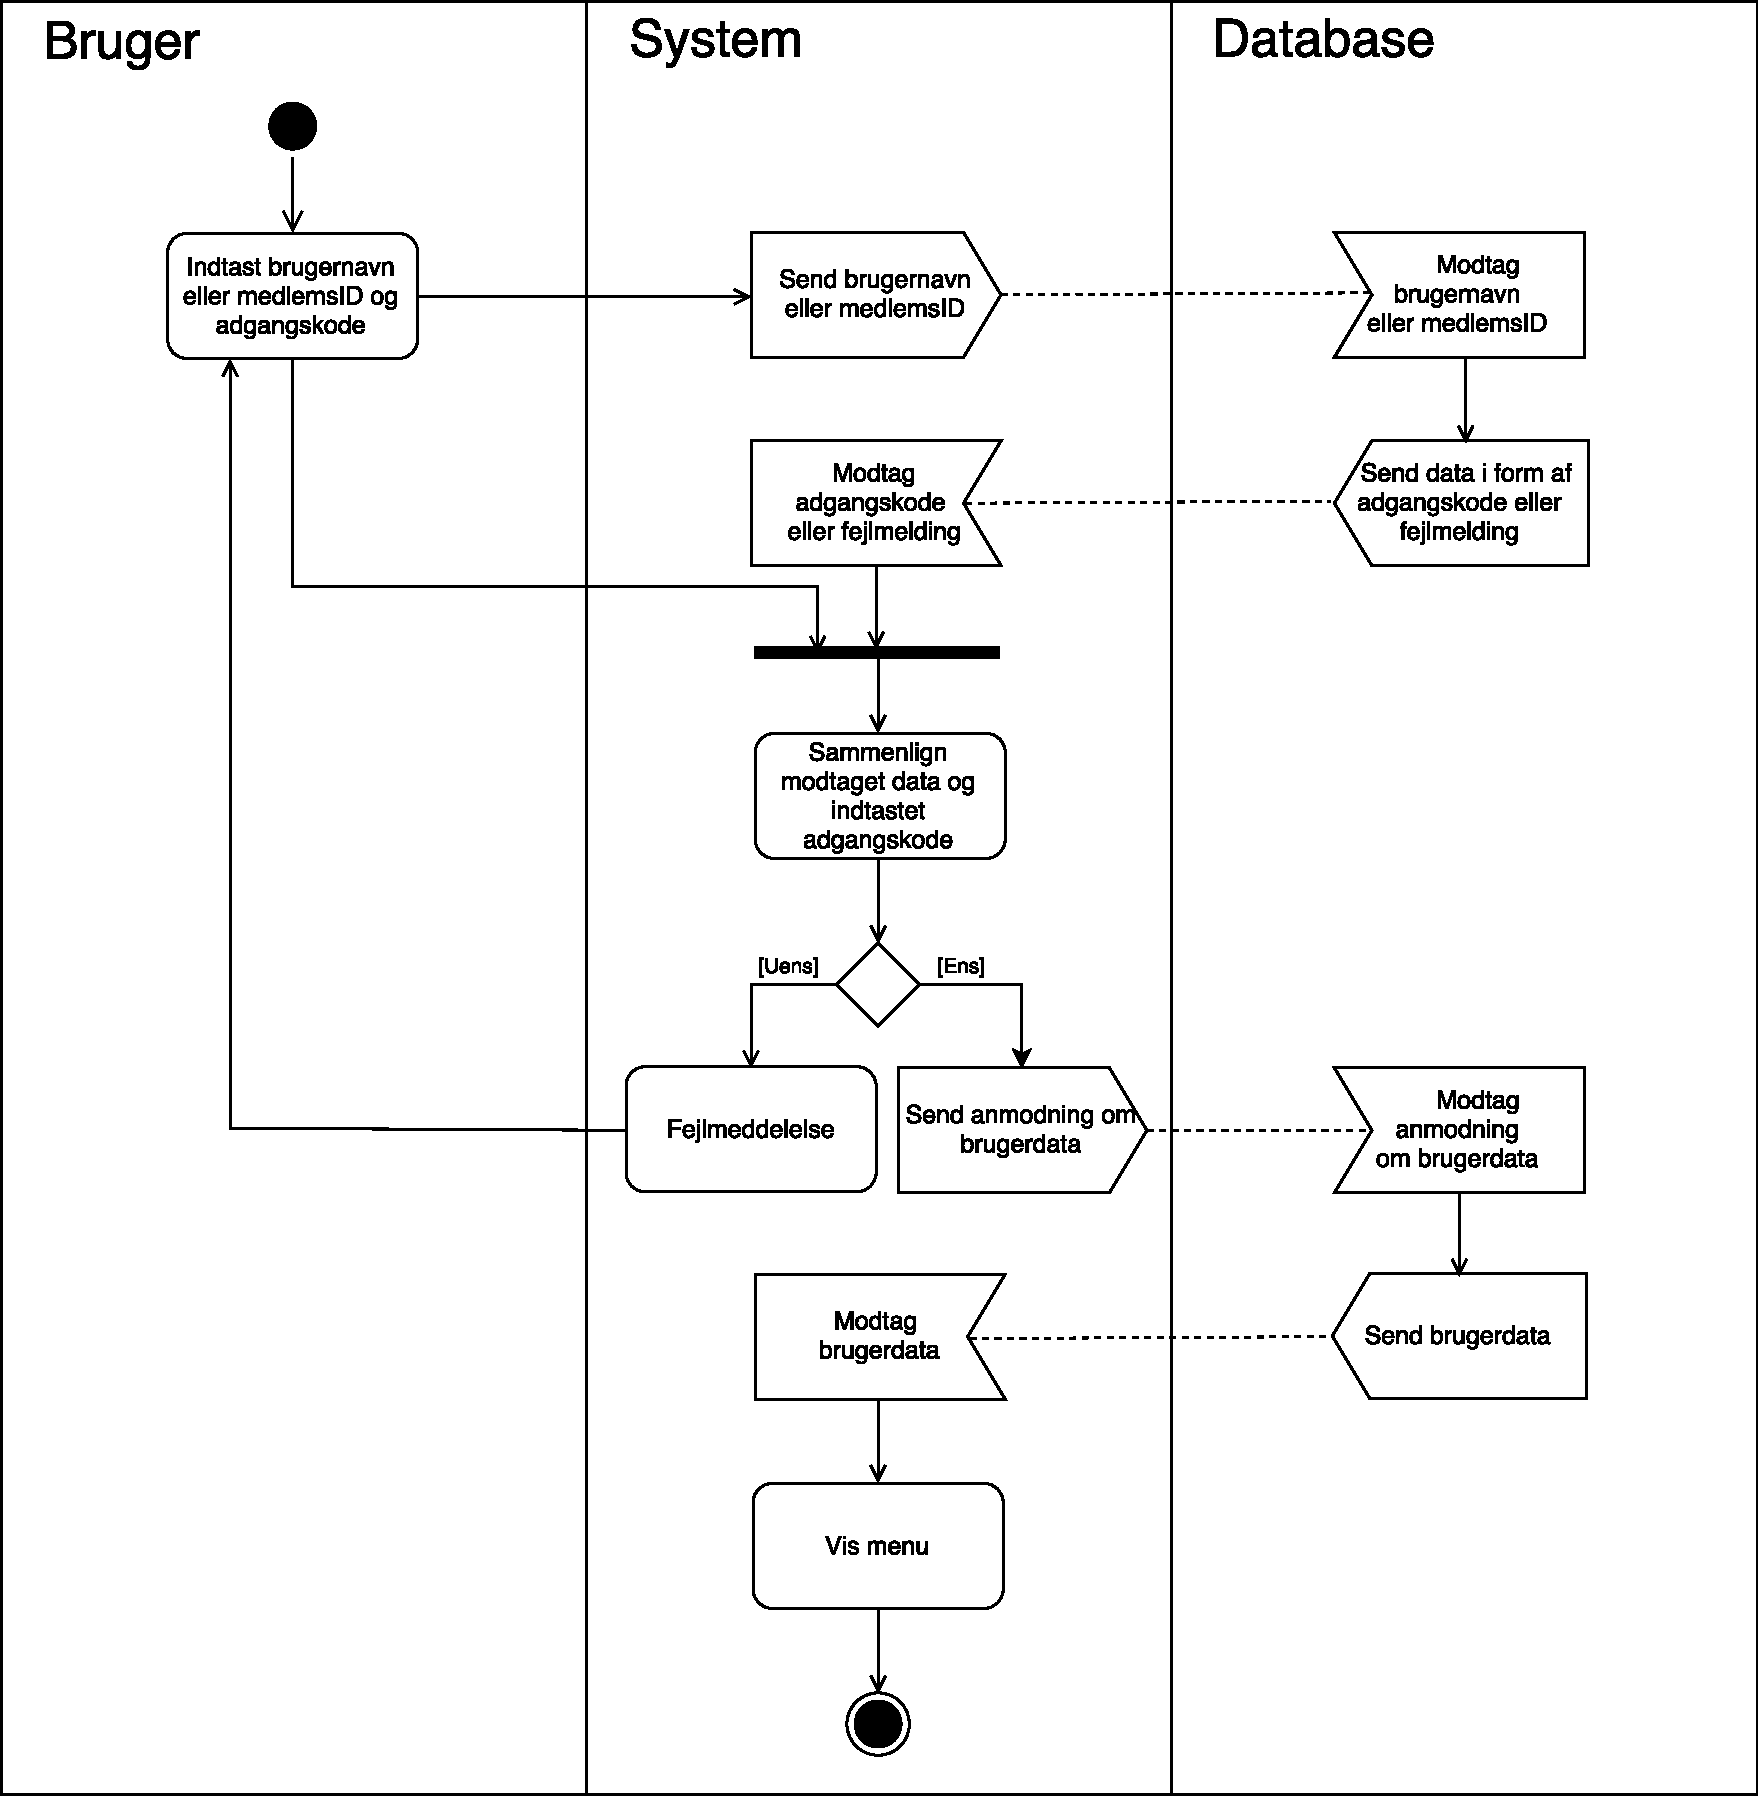
\includegraphics[width=0.9\textwidth]{figures/aktivitetsdiagram/Logind}
\caption{Aktivitetsdiagram over log ind.}
\label{fig:logind}
\end{figure}



